%
% Szakdolgozatminta az Eszterházy Károly Katolikus Egyetem
% matematika illetve informatika szakos hallgatóinak.
%

\documentclass[
% opciók nélkül: egyoldalas nyomtatás, elektronikus verzió
% twoside, 	% kétoldalas nyomtatás
% tocnopagenum,% oldalszámozás a tartalomjegyzék után kezdődik
]{thesis-ekf}
\usepackage[T1]{fontenc}
\usepackage{graphicx}
\PassOptionsToPackage{defaults=hu-min}{magyar.ldf}
\usepackage[magyar]{babel}
\usepackage{mathtools,amssymb,amsthm,pdfpages}
\footnotestyle{rule=fourth}

\newtheorem{tetel}{Tétel}[chapter]
\theoremstyle{definition}
\newtheorem{definicio}[tetel]{Definíció}
\theoremstyle{remark}
\newtheorem{megjegyzes}[tetel]{Megjegyzés}

\begin{document}
	
	\institute{Matematikai és Informatikai Intézet}
	\title{Játékfejlesztés Unity keretrendszerben}
	\author{Rokob Attila Adrián\\Programtervező Informatikus}
	\supervisor{Troll Ede\\tanársegéd}
	\city{Eger}
	\date{2025}
	\maketitle
	
	\tableofcontents
	\chapter*{Bevezetés}
	\addcontentsline{toc}{chapter}{Bevezetés}
	
	Még annak idején, éppen hogy óvodából kikerülve volt az első alkalom, hogy játszottam bármi féle számítógépes játékkal. Még olvasni alig tudtam, első betű amit megjegyeztem, az a "C" volt, hogy el tudjak jutni a Cartoon Network, saját, Flash játék oldalára, tele volt végtelen sok, alacsony költségvetésű játékkal, minden féle Cartoon Network IP alapján. Egy Mario Maker szerű Ben 10 Platformer, egy astroboy shoot em up, Egy Johnny test top-down shooter.
	Közel már ekkor eldöntöttem, hogy én, ha nagy leszek, játékokat fogok fejleszteni. Amint el végeztem az általános iskolát, emiatt is mentem egyenesen tovább egy informatikus középiskolába. Ebben a középiskolában íram meg az első tényleges sor kódomat, egy c\# tömb kiírót, GOTO kifejezéssel, mivel még nem tudtam róla, hogy hogyan működnek a ciklusok. Ezen felüll ebben az iskolában jöttem rá, mennyire élvezhető is maga a kód írás, mennyi kreativitást lehet felhasználni, egy ennyire strukturált médiumban is.
	Miután végeztem közép iskolával, illetve egy covid alatti szoftverfejlesztő képzéssel, természetesen egyből jött is az egyetem, akkor már inkább egy stabil, viszonylag stresszmentes karrier által motiválva.
	Itt egyetemen készült el az első, befejezett (illetve annak mondott) Unity játékom, egy, a konzulensem Troll Ede tanárúr által rendezett Game Jam-re készített kalózos, társasjáték.
	Ennek a projektnek a készítése során Tanultam meg a szakdolgozatom alapját is adó Unity játékmotor alapjait. Ezek után már eléggé egyértelművé vált számomra, hogy a szakdolgozatomat is szeretném, hogy egy játék legyen, és mivel Unity-vel már volt tapasztalatom, illetve nem mellékesen továbbra is vezeti a piacot kissebb költségvetésű játékoknál.
	Magának a projetktnek, a tematikája eredetileg még a Leányka Bisztró egyik kanapéján dőlt el, hogy legyen fél úton egy "kalózos For The King", és egy "cyberpunk Nuclear Throne" között. Mivel eredetileg Gyökösi kata feladata volt az univerzum, illetve az egész játék kinézetének létrehozása, ezért maradtunk a kalóz tematikánál. Mivel a játékmenet létrehozása az én feladatom volt, emiatt maradtunk Nuclear Throne szerű felül nézetes, lövöldözős játékmenetnél, illetve idő hiánya miatt a Rogue Like elemek hozzáadásánál, mint például a véletlen generált világ, ellenfelek, és szint végén kapható tárgyak.
	
	
	\chapter{Technológiai Bevezetés}
	\section{Godot bemutatása}
	\subsection{Főbb jellemzők}
	A godot Engine egy multi platform, ingyenes, nyílt forráskódú játékmotor. Életét egy zárt forráskódú, "Larvotor" nevű motorként kezdte, argentin játékfejlesztő cégek számára, 2001-ben\cite{GodotInImages}.
	Első nyilvános verzióját 2014-ben adták ki GitHub-ra, egy MIT licensz\cite{MITLicense} alatt. 2016-ban 20000\$ támogatást nyert el a Mozilla Open Source Support "Mission Partners" Programjának keretében, Web Sockets, WebAssembly, és WebGL 2.0 támogatás hozzáadása céljából.\cite{MOSS}
	
	Nevét a Samuel Beckett, francia "Godotra várva"\cite{GodotraVarva} könyvről kapta. A könyvben kettő karakter a címzetes Godotra várnak, aki viszont nem érkezik meg. Ezt a játékmotor eredeti készítői, Juan Linietsky és Ariel Manzur hasonlítják ahhoz, ahogyan szoftver fejlesztők keresik a tökéletes megoldást, a tökéletes kódot, ami ahogy a könyvben, úgy a szoftverfejlesztésnél sem érkezik sosem.\cite{GodotInImages}
	A godot 3.0 egy közel teljes refaktorálást igényelt, hogy lehetővé tudja tenni a rendering-pipeline újradolgozását.\cite{Godot3} Nem sokkal ez után a verzió után létre hoztak egy Patreon oldalt, amely lehetővé tette hogy a kettő eredeti fejlesztő teljes munkaidőben tudjon dolgozni a motor fejlesztésén. 2019-ben a fejlesztői csoport két részre bomlott. Míg Linietsky csapata a jövő béli 4.0 ággal foglalkozott, Verschelde csapata a 3.0 branch fenntartását kezelte. A 4.0 verzió ismételten újra írta a motor magjának jelentős részét, hogy frissebb hardver lehetőségeket ki tudjon használni, mint például a több szálon futó kódot.\cite{Godot2022}
	
	A motor 4.0 verziója 2023-ban lett kiadva. Ebben a verzióban adtak hozzá támogatást a Vulkan rendering API-hoz, illetve sokkal optimalizáltabbá tették a GDScript-et, és a beépített renderer-t is.\cite{Godot4}
	Íráskori legfrissebb verziója a Godot 4.4, amely sok régóta várt funkciót hozzáadott a motorhoz, például fizikai interpolációt, egy fejlettebb beépített fizikai motort, és játékon belüli szerkesztést.\cite{Godot44}
	
	A Godot-ban minden játék egy Node\cite{GodotKeyConcepts} alapú fa hierarchia, ahol minden vissza vezet az úgy nevezett root node-ra\cite{GodotKeyConcepts}. Ez a node tartalmazza magában beágyazva a játék összes részét.
	Több node gyűjteménye hoz létre egy Scene-t\cite{GodotKeyConcepts}, ami egyfajta tároló al-Node-oknak, újrafelhasználhatóság érdekében. Például egy Player Scene valószínőleg tartalmazni fog magában egy Sprite-ot, egy Collidert, és egy Script-et, ami mozgatja a karaktert.
	Ezen felül minden node közti kommunikáció Signal-ok\cite{GodotKeyConcepts} formájában történik. Ezek egy szintnyi absztrakciót adnak hard kódolt eventek felett. Például, hogyha meg nyomunk egy gombot, ami megnyit egy menüt, se a menünek nem kell tudnia, hogy melyik Node nyitotta meg, se a gombnak, hogy mit csinál az a signal, amit meg hív. Ezen felül számos beépített Signal is van, például, hogy kettő collider ütközött, vagy egy node-ot megsemmisítettek. A signal rednszer a Godot vezriója egy Observer Pattern-nek.\cite{ObserverPattern}
	A Godot-ban minden kód* egy saját fejlesztésű nyelven, a GDScript-ben\cite{GDScript} íródik. Ez a nyelv a godot-hoz hasonlóan objektum orientált, illetve imperatív, tehát azt írja le hogy *hogyan* érjük el a célunkat, ahelyett, hogy *micsoda* a cél. A nyelv fokozatosan típusos\cite{GradualTyping}, ami ezt jelenti, hogy valahol a gyengén, és erősen típusos nyelvek között helyezkedik el. Minden értéknek kell, hogy legyen egy típusa, viszont van egy beépített "dynamic"\cite{godotDynamicKeyword} típus is, ami lehtővé teszi hogy az érték típusa csak futási időben legyen meghatározva.
	Legismertebb játékok, amelyek ezt a motort használják: Dome Keeper \cite{domeKeeperEngine}, Brotato \cite{brotatoEngine}, és a Cruelty Squad \cite{crueltySquadEngine}
	\subsection{Unity keretrendszerhez képest}
	A Godot motor főbb előnyei Unity-hez képset, sokkal magasabb szintű modularitás, a Node rendszernek köszönhetően, illetve az MIT licensznek köszönhetően a nyílt szabad felhasználás.
	Főbb hátrányai Unity-hez képest, egy sokkal kissebb, kevésbé tapasztalt közösség, illetve még mái napig fejlesztés alatt álló 3D képességek.
	
	
	\section{Unreal bemutatása}
	\subsection{Főbb jellemzők}
	Az Unreal Engine a világ második legnépszerűbb játékmotorja\cite{unrealPopularity}, életét 1998-ban kezdte egy Unreal nevű, elsőszemélyű nézetes, lövöldözős játék fejlesztésére használt motorként. A készítője, Tim Sweeney, akkori Epic Megagames, jövőbéli Epic Games vezérigazgatója \cite{aboutEpicGames}, már a játék készítésének elejétől fókuszált a játék készítésre használt eszközök fejlesztésére, ezzel elősegítve, hogy a motort, bárki komplett termékként is tudja használni.
	
	Az Unreal egy nyílt forráskódú, de kereskedelmi céllal írt szoftver.\cite{unrealLicense}  Epic Games, a tulajdonos/ fejlesztő cég a motor mögött egy millió dollár bruttó bevétel után 5\%-os részesedést igényel, kivéve abban az esetben, hogyha a terméket kizárólag az Epic Games Store-on adják ki a fejlesztők.\cite{unrealPopularity}
	
	A motor első, Unreal fejlesztésére készített verziója az Unreal Engine 1 (akkoriban még csak Unreal Engine) 1998-ban került kiadásra. Első verziója kizárólag szoftveres renderelést támogatott, többszörös újra írás után viszont több hardver rendering API-t is tudott használni. Ezen felül még fontos megemlíteni a valós idejű szint-geometria szerkesztőt is, hiszen kortársai közül egyik első volt, hogy ezt a lehetőséget nyújtsa. Ezzel a verzióval készült el az Unreal Tournament, egy online, kompetitív verziója a kmotor nevét adó játéknak.
	
	Következő fő verziója, a 2002-ben kiadott Unreal Engine 2.0\cite{unreal2Released}, át tette a fókuszát otthoni konzolokra való fejlesztésre, a számítógépes játékokon felül. \cite{historyOfUnreal} Ezen felül a rendering motor, az első verzióval ellentétben, elejétől kezdve hardveres renderelésen alapult. A motornak ez a verziója volt az első, hogy támogassa a DirectX 8-at. Az Unreal Engine 2 a Karma fizikai motort használta.
	
	3.0 legelső verzióját 2004-ben adták ki. Főbb előrehaladás volt a motor életében egy új, és sokkal erősebb fizikai-, hang- illetve renderelő rendszer. \cite{anEpicNextGenAdventure} Ezt a verziót elejétől fogva, teljesen programozható shader hardverre írták, ami ennek idejére már elterjedté vált. Ezen felül egyik első játékmotor volt, ami támogatta a több szálon történő szoftver futtatást.\cite{unrealMultithreaded} Továbbá első verzió volt, ami a DirectX 9-et használta alap grafikai API-nak, lehetővé téve a sokkal feljettebb Vertex- és Pixel Shaderek használatát.
	
	4.0 legnagyobb előrelépései egy teljesen lecserélt kódolási rendszer \cite{unrealBlueprint}, és a fizikai alapú renderelés hozzáadása volt.
	
	A motor 5.0 verziója legfőképp vizuális irányban tett előrelépéseket, kettő legfőbb előrelépés, a ,,Nanite'', illetve a ,,Lumen'' voltak. A Nanite Egy technológia, amely lehetővé teszi fejlesztőknek, hogy akármekkora részletességgel töltsenek fel modelleket a motorba, minden egyszerűbb modellt a motor maga generál, valós időben. A Lumen egy teljesen dinamikus, valós idejű, fénykezelő rendszer, lehetővé teszi sokkal élethűbb jelenetek megjelenítését játékok számára.
	
	Néhány említésre méltó Játék, amit Unreal-lel készítettek a Black Myth: Wukong \cite{wukong}, a Sea of Thieves \cite{seaOfThieves}, és a Fortnite \cite{Fortnite}
	
	\subsection{Unity keretrendszerhez képest}
	Főbb előnyei Unityhez képest egy sokkal fejlettebb, kidolgozottabb alap render pipeline, illetve egy gráf alapú kódolási környezet.
	
	Főbb hátrányai legfőképp a nehezebb tanulhatóság, alacsonyab platform függetlenség, és jobb grafikából eredő teljesítmény csökkenés
	
	\section{Unity bemutatása}
	\subsection{Főbb jellemzők}
	
	A Unity a világ legelterjedtebb motorja, főleg kisebb költségvetésű játékok esetében.\cite{unrealPopularity} Életét 2004-ben kezdte, három dán ember kezében. Ez a három ember David Helgason, Joachim Ante, és Nicholas Francis volt. A motort legfőképp kisebb, független fejlesztőknek készítették, akiknek nem voltak erőforrásai, a nagyobb motorok licenszeléséhez. 2005-ben megérkezett első verziója, kizárólag Max Os X-re, egyből sikeres is volt a célközönségével. Miután kiadták ezt a verziót, egyből vettek is fel embereket, frissítették, pontosították a dokumentációt, új funkcionalitást adtak a motorhoz, illetve támogatást adtak akkori felhasználóiknak.
	
	A motor 2.0 verzióját 2007-ben adták ki. Ennek a verziónak legfőbb részei a beépített hálózatkezelés, terep generációs motor, dinamikus árnyékok, és videó visszajátszás voltak. Ebben a verzióban vált először támogatottá a Windows, és a web alapú játékok fejlesztése.
	
	Következő, harmadik verziója 2010-ben érkezett meg, magával hozott egy fejlettebb grafikai motort számítógépekre, és konzolokra, beleértve lehetőséget késleltetett kijelzésre való lehetőséget, egy harmadik fél fénytérképező eszközének integrációját, natív betűtípus kijelzőst, és automatikus UV térképezést. Ez volt az első ingyenesen elérhető verziója, személyes, illetve oktatói céllal.
	
	A 2012-ben kiadott 4.0 hozzá adott egy ,,Mecanim'' nevű animációs keretrendszert, komplexebb, élethűbb animációk létrehozása érdekében. Fontos még említeni, hogy ez volt az első verzió, amely támogatta az Asset Store-t, egyfajta játékelem piacot. Ez összekötötte a különböző komponensek készítőit, és felhasználóit, tovább zökkenőmentesítve játékelemek beszerzését. Ez a verzió volt az első, ami Linux-ot, illetve Adob Flash Player-t támogatta.
	
	A Unity 5.0 2015-ben jelent meg, Unity Services-zel együtt. A Unity Services egy felhő alapú szoftver eszköztár, benne előre megírt autentikációs, bevételkezelési, vagy akár teljes szerver üzemeltetési lehetőségekkel fejlesztők számára. Ez volt az utolsó Unity verzió, mielőtt a motor át állt kiadás évén alapuló verziókra.
	
	A Unity 2017, és 2018 hozzáadott a motorhoz egy kód szerkszthető Render Pipeline-t, három különböző verzióval, egy Lightweight (Könnyűsúlyú) mobil eszközökre, egy Universal (Univerzális) minden platformra, és egy High Definition (Részletes) kiemelten magas teljesítményű eszközökre, mint egy konzol vagy számítógép, vagy akár előrenderelt projektekhez. Ezen felül még megérkezett ezt a rendszert támogató Shader-, és Visual Effect Graph, egy shader, illetve vizuális hatás készítést elősegítő absztrakció, Machine Learning Agent, mesterséges intelligencia képzésére készített komponens, Entity Component System, egy projekt rendezési minta, Jobs System, többszálaszítás egyszerűsítése érdekében, és a Data-Oriented Technology Stack. 
	
	Következő két év verziói a stabilitáson, illetve hatékonyságon fókuszáltak. Az Incremental Garbage Collection, azaz lépcsőzetes szemét gyűjtés, elkerüli a memória felszabadításával járó akadásokat, a Burst Inspector mélyebb belátást ad a már optimalizált kód működésébe, a DOTS Runtime Debugger, és Live Link segítettek futásidőben bele látni a kód működésébe, illetve valós idejű szerkesztésben, DOTS NetCode, pedig egyszerűsítette többjátékos játékok készítését. \cite{historyOfUnity}
	
	Az írás pillanatában legújabb Unity verzió, a Unity 6. Ez a verzió további teljesítmény előrelépéseket ért el, ezek a GPU Resident Drawer, jobban kihasználva modern videókártyák kötelgelt renderelési készségeit, GPU Okklúziós Selejtezés, többször feldolgozott pixelek csökkentésére, és a Spatial Temporal Post-Processing, egy multi platform felbontásnövelő. \cite{unity6IsHere}
	
	Néhány említésre méltó játék, ami ezzel a motorral készült a Hearthstone \cite{hearthstone}, a Rust \cite{rust}, és a Beat Saber \cite{beatSaber}.
	
	\subsection{Miért a Unity-t választottam}
	Legegyszerűbbnek úgy tartom elmagyarázni, azt, hogy miért a Unity-t választottam, hogy elmagyarázom miért nem a konkurencia mellett döntöttem.
	
	Kezdeném az Unreal-lel. Ő mellette a legnagyobb ellenérvem, amikor elkedztem a projektet, az volt hogy túl komplex, túlságosan 3D-re kiélezett, ahhoz, amit én szerettem volna elérni. Gyönyörű szép, intuitiv render pipeline-nal nem megyek messzire, hogyha a játékom kinézete egy 30 éves konzolon sem lett volna kiemelkedő, főleg abban az esetben, hogyha ez teljesítménybe és fejlesztési időbe is kerül.
	
	Godot ellen legnagyobb érvnek, főleg projekt kezdés idejében azt tudnám mondani, hogy mennyire fiatal még a motor, mennyire sok extra, kényelmi funkció hiányzik belőle, amit a unity-ben alapértelmezettnek veszek, például a Pixel perfect kamera, vagy a részecskefizikának néhány komplexebb része.
	
	Legfőképp ugye ez a kettő olyan motor volt, konkurens, de szeretném még megemlíteni a GameMaker-t is, hiszen ahogyan arra utólag rájöttem, nagyjából direkt az én játékomra faragták, és a projekt legnagyobb inspirációja, a Nuclear Throne is ezt a motort használja. Viszont ő vele a legnagyobbik probléma csak az volt, hogy arra, hogy egy teljesen kompetens motor, rájöjjek, addigra már közel kész voltam az egész játékkal.
	
	Összesítve úgy érzem, jó döntést hoztam motor terén, nem volt olyan dolog, amit elvártam volna a Unity-től, ami kifogott volna rajta, esetleges véletlen, végtelen ciklusokat leszámítva.
	
	\subsection{Használt Unity komponensek bemutatása}
	
	\subsubsection{Collider, Rigidbody}
	%TODO: döntsd el, hogy kell-e neked collider, rigidbody leírás
	
	\subsubsection{Tilemap, Tilemap Extras}
	A Tilemap, mint ötlet, azt írja le, hogy egy mátrixra bontjuk le a játékteret, hogy ezzel egyszerűsítsük magának a világnak a létrehozását.
	A mátrixon felül, minden Tilemap-nek tartalmaznia kell egy Tileset-et is. Ebben az előre létrehozott listában, van eltárolva az összes lehetséges érték, amit fel tud venni egy pozíció a mátrixon belül. A mátrix pozíció, és a kiválasztott érték kombinációját hívjuk csempének.
	
	A Tilemap, mint Unity-n belüli csomag, ennek az ötletnek egy előcsomagolt kidolgozása. Tartalmaz egy előre megírt, szerkeszthető, kibővíthető Tilemap komponenst, és minden egyéb részt, ami ennek a komponensnek a használatát segíti, például egy Tile Brush-t, könnyebb csempe lehejezés érdekében, Tilemap Collider, ütközés optimalizálás céljával, illetve egy úgymond vászonként használható Grod komponenst.
	\subsubsection{Régi és Új Input rendszer}
	A Unity régi input rendszere volt az eredeti, már az első verziója részeként lett hozzáadva. Még továbbra is a motor alapértelmezett beneneti rendszere. Az Input osztályra épül, ebben az osztályban van tárolva az összes használathoz szükséges metódus. Nem használ eseményeket, hanem ehelyett minden képkockán ellenőrzi, a bemeneti értékeket, ezen felül pedig közvetlenül kötött a bemeneti művelet, az eszköz típushoz, amiből a bemenet érkezik. Ez azt jelenti, hogy nincs beépített támogatás kettő, egyező típusú eszközre.
	
	Az Input System csomag, más nevén az új bemeneti rendszer régi társának hibáit kijavítva 2019-ben jelent meg. Régi redszerrel ellentétben eseményeken alapszik, nem kérdezi le az összes eszköz állapotát, minden képkocka esetében.  Ezen felül még előrelépés az is, hogy több osztályra alapszik, mivel magasabb szintű absztrakcióval rendelkezik. Ez az absztrakció abban nyilvánul meg, hogy a bemenet, hogy mit csinál, és a bemeneti eszköz között van még egy szint, az InputAction. Ez a szint képes kezelni akár több bemeneti eszközt is, akár ugyanarra a műveletre is. Ez azt jelenti, hogy ezzel a bemeneti rendszerrel tudunk egy játékost egyszerre akár több eszközzel is irányítani, és ezzel a rendszerrel már lehetséges több, egyező típusú irányító hardver különválasztása is.
	
	
	\subsubsection{Testing Framework}
	A Testing Framework egy Unity által készített külső csomag, NUnit-nak egy kiterjesztett verziója, kiemelten játékok tesztelésére kiélezve. Minden ilyen módon írt tesztet két csoportba tudunk sorolni. Első csoport ezek közül a szerkesztői tesztek. Ezek a tradicionális, egyből, és egy szálon futó, játék elindítását nem igénylő tesztek. Ezeken a testing framework csak apróbb dolgokat változtat, például futtathatóvá tesz coroutine-okat a teszteken belülről, egy attribútum segítségével. Ilyen teszteket például egy matematikai függvény tesztelésére, vagy egy útkereső algoritmus ellenőrzésére lehetséges használni. Szerkesztői teszteken kívül még léteznek játék béli tesztek, amit a Unity Testing Framework ad hozzá az NUnit-hoz. Ezek a tesztek tényleges, játékon belüli eseteket ellenőriznek, például hogy a játékos tud-e mozogni, vagy hogy a világ, generálás után követelményeknek meg-e felel.
	
	\chapter{Rendszerterv}
	\section{Bevezetés}
	Ez a dokumentum azzal a céllal jött létre, hogy bemutassa, dokumentálja Rokob Attila Játékfejlesztés Unity keretrendszerben szakdolgozatára készülő játékát.
	
	\section{Fő ötlet}
	A játék egy felül nézetes, lövöldözős, roguelike \cite{roguelike} játék, ami mögötti legnagyobb inspirációk a Nuclear Throne \cite{nuclearThrone} villámgyors játékmenete, és véletlenszerűen generált előrehaladása, illetve a kalóz fantázia szeretete
	
	\section{Megkülönböztető jellemzők}
	\subsection{Minden menet különböző}
	A világ, ahol a játékos fog tudni közlekedni, minden indításnál frissen, véletlenszerűen generálódik. Minden így generálódott világot csomópontok építenek fel. Ezek a csomópontok egy reprezentációi egy játékon belüli "kör"-nek. Alap, Elite és Boss Csomópont harcot jelent, aminek a végén a játékos kap aranyat, illetve választhat 2 tárgy közül. A Bolt Csomópont lehetőséget ad a játékosnak, hogy egy felugró ablakban elköltse a keresett aranyát különböző tárgyakra.
	
	\subsection{Komplex ellenfelek}
	Ellenfelek képesek lesznek komplex döntéseket hozni, egy fejlett döntési fa alapján. Több frakcióból származó ellenfél nem csak a játékossal fog tudni harcolni, hanem egyéb ellenfeleivel is. Ezen felül minden ellenfél típusnak külön módja lesz a döntés hozatalra, egy közelharcos kutya sokkal jobban fog közeledni a célpontjához, mint egy muskétás. Ezen felül ellenfelek mozgásai- és támadási viselkedése külön lesz választva egymástól, hogy ezzel is csökkenjen a coupling.
	
	\subsection{Tárgyak}
	Egy meccs folyamán a játékos fő előrehaladási módja különböző tárgyak szerzése lesz. Ezek a tárgyak változatos bónuszokat adjak a játékosnak, mint például nagyobb sebzést, célkövető lövéseket, vagy akár egy teljesen új fegyvert. A tárgyak kiegyensúlyozottság érdekében különböző osztályokba lesznek sorolva, attól függően, hogy mennyire nehéz őket megszerezni. Ezek az osztályok a következőek lesznek:
	A legalacsonyabb erejű tárgyak alap csomópontokból lesznek megszerezhetőek, ők lesznek a leggyakoribbak. Ilyen tárgyak esetek nagy részében csak a játékos számait változtatják majd, például hogy mennyit sebez egy lövés, vagy hogy mennyi a maximális élete.
	A következő szint a boltból megszerezhető tárgyak, akik legtöbbször nem fognak kihatni közvetlenül a harcra, hanem egyéb módon adnak segítséget a játékosnak, például egy kedvezményt adnak jövő béli boltokban vagy lehetségessé teszik a játékos számára, hogy kihagyjon egy csomópontot, vagy átugorjon a világon máshova.
	Harmadik szintű tárgyakat elit csomópontokból lehet megszerezni, tehát nem lesznek túl gyakoriak, viszont cserébe az összes ilyen tárgy nagy mértékben változtatni fogja a játék menetét. Ilyen tárgyak adhatnak a játékosnak lövedék duplázást, élet lopást, vagy akár lehetőséget újjászületésre is.
	A legritkább, és ezzel a játékra legnagyobb kihatással lévő tárgyakat minden világ végén lévő Boss fogja dobni. Minden ilyen tárgynak legalább egy pozitív és legalább egy negatív hatása is lesz. Ilyen tárgyak adhatnak a játékosnak óriási életlopást, negatív élet regenerációért cserébe, vagy akár megakadályozhatják hogy a játékos célozzon de cserébe tűzgyorsaságot, és célkövetést adnak minden lövésének.
	
	\section{Egyéb rendszerek}
	\subsection{User Interface}
	A játék tartalmaz egy fő menüt, ahonnan el lehet indítani a meccseket, be lehet állítani a generálómagokat, hogy mindig ugyanaz a világ legyen legenerálva, illetve ki lehet lépni a játékból.
	Ezen felül a játékos életét meccsen belül végig lehet látni, akár a világban, akár egy csomóponton van a játékos.
	A játékot meg lehet állítani, előhozva egy menüt, ahol folytatható a játék, vagy ki tudunk belőle lépni.
	Amikor a játékos nincsen egy csomóponton belül, tud aranyat költeni arra, hogy gyógyítsa magát, az ezt lehetővé tévő user interface elérhető ilyen helyzetekben.
	Ezen kívül ugyanebben a helyzetben a játékos meg tudja nézni jelenleg milyen tárgyak vannak, ezeket ki és be tudja kapcsolni.
	Minden csomópont végén lesz egy láda, amivel el lehet érni egy tárgy választó ablakot, ebből a játékosnak ki kell tudnia választania hogy melyik tárgyat szeretné.
	\subsection{Elkülönített véletlen szám generátorok}
	Mivel a játék egy generálómagon alapszik, de elérhető kell hogy legyen a véletlen szám generátor a játékon belül is, ezért külön kell választani több szálra ezt.
	Jelenleg ezek a szálak vannak meghatározva:
	A fő világ által használt szál: Ezt semmi más nem tudja használni, úgy hogy több világot is lehessen generálni vele, újraindítás nélkül. Felhasználásra példa: Világon hol legyenek csomópontok, melyik csomópont, melyikhez kötődjön.
	Csomópontokon belüli szál: Ezt minden csomópont elején újra létre kell hozni, a csomóponthoz hozzárendelt generálómag alapján, csak az az egy csomópont használhatja, aki készítette, és csak a csomóponton belüli dolgok eldöntésére Felhasználásra példa: csomópont végi ládában milyen tárgyakból lehessen választani, milyen kiosztása legyen a csomópontnak, hány, és milyen ellenfél idéződjön benne.
	Vizuális Különbségek szál: bárhol használható, ahol csak a játék kinézetére fog kihatni. Felhasználásra példa: világ térképen pontosan hol jelenjenek meg a csomópontok, ellenfeleknek-, csempéknek melyik kinézete legyen leidézve.
	
	\section{Fejlesztési idővonal}
	
	
	\chapter{Saját projekt fejlesztése}
	Ebben a fejezetben lesz kifejtve a tényleges projektem. Alfejezetek amiatt vannak ilyen furcsa sorrendben, mivel lehetőség szerint minden csak az előtte már kifejtett dolgokon alapul
	\section{Interfészek}
	\subsection{IDealsDamage}
	Az IDealsDamage, lehetővé teszi akármilyen objektumnak, hogy meg próbálkozhasson sebezni egy másik célpont játékobjektumnak. Fontos megjegyezni, hogy sebzésre módot nem tartalmaz az Interfész, kizárólag egy TryToDealDamage (próbálj meg sebezni) metódust.
	

	\begin{figure}
		\centering
		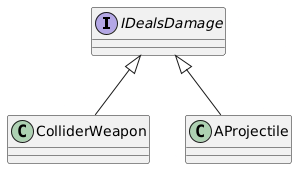
\includegraphics[width=0.5\linewidth]{ImplementsIDealsDamage}
		\caption[IDealsDamage implementációi]{IDealsDamage implementációi}
		\label{fig:implementsidealsdamage}
	\end{figure}
	
	\subsection{IInteractable}
	Ez az Interfész ezt jelzi, hogy a játékos interakcióba tud lépni az implementáló osztály objektumával. Egyetlen Interact metódust tartalmaz.
	
	\begin{figure}
		\centering
		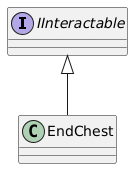
\includegraphics[width=0.25\linewidth]{implementsIInteractable}
		\caption[IInteractable implementációja]{IInteractable implementációja}
		\label{fig:implementsiinteractable}
	\end{figure}
	
	\subsection{IRandomStream}
	Az IRandomStream egy absztrakciója a különböző random stream-eknek, ezeknek egyszerűbb kezelése érdekében. Magába foglalja az összes metódust, amelyről elvárt, hogy minden random stream implementálja, ami ebben az esetben csak a Range metódus 2 variánsa, egy egész, és egy lebegő pontos szám alapú.
	
	\begin{figure}
		\centering
		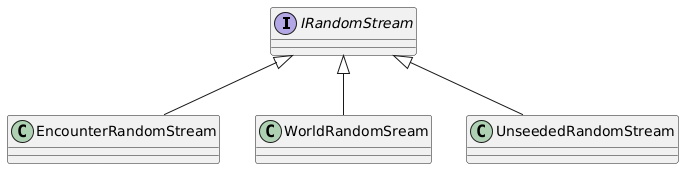
\includegraphics[width=1\linewidth]{implementsIRandomStream}
		\caption[IRandomStream implementációi]{IRandomStream implementációi}
		\label{fig:implementsirandomstream}
	\end{figure}
	
	\section{Random Streams}
	Mivel a Unity beépített Random osztálya \cite{unityRandom}, a System beépített random osztályával \cite{systemRandom} ellentétben statikus, ezért hogy több szálon tudjon futni (megadott, és nem megadott generáló magú), létre kellett hozzak egy kezelő osztályt. Ebben az osztályban van eltárolva minden különálló szál legutóbbi állapota, illetve ez az osztály kezeli az állapotok megfelelő betöltését használat előtt, és eltárolását használat után. Ezen felül az osztály elérhetővé teszi saját, wrapper függvényein keresztül a különböző szálak megfelelő használatát.
	\section{VectorWrappers}
	Kódolás gyorsítása, illetve Type Safety (Típus biztonság) érdekében a projekt közel teljesen elkerüli a Vector3 \cite{unityVector3}osztály közvetlen használatát, helyettesíti őket általam írt wrapper osztályokkal. A projekt megvalósítása 3 különböző vektor wrapper-t igényelt.
	\subsection{UnnormalizedVector3}
	Ahogyan az osztály nevében is szerepel egy normalizálatlan 3 dimenziós vektor. A projekten belül legfőképp pozíciók reprezentációjára használtam.
	\subsection{NormalizedVector3}
	Egy normalizált vektor osztály, kizárólag normalizált értékeket tud eltárolni, illetve visszaadni.Ezt az osztályt a projekten belül legfőképp különböző irányok meghatározására használtam.
	\subsection{NodeVector3}
	Egy speciális vektor wrapper, azzal a céllal, hogy az útkereső algoritmus könnyebben tudja a játék teret négyzetrácsos mátrixszá bontani, hogy lehessen rá alkalmazni az A* algoritmust. Ezt a felbontást először is azzal érjük el, hogy a z koordináta nem tud nullán kívül semmi más értéket felvenni, illetve hogy az x és a z koordináta csak -0.5, 0, vagy pedig +0.5 értéket tud felvenni.
	% TODO: vizualizáld a 9 lehetséges értéket a vektorhoz
	\section{VisionChecker}
	Egy segéd osztály, ami az ellenségek látás vonalát kezeli. Vet egy sugarat a kettő megadott pozíció között, és attól függően, hogy először falat, vagy játékost talál el, vissza adja, hogy látható-e a játékos a felhasználó pozíciójából.
	\section{A* Pathfinding}
	\subsection{Algoritmus bevezetése}
	Ennek az algoritmusnak alapja a teljes út két részre bontása, és ezek alapján történő iteráció, a legalacsonyabb költségű utat keresve. Első fele ennek a költségnek az eddig megtett lépések tényleges költsége. A másik fele a költségnek egy tipp, arról hogy a jövőbéli lépések összege mennyi lesz egy úgynevezett heurisztikus függvény alapján. Ennek a függvénynek optimalizálása egyik, ha nem a legfontosabb része az algoritmus hatékonyságának növelésében.
	
	Iteráció először mindíg csak az előreláthatólag legalacsonyabb költségű csomóponton történik, ezzel eliminálva nagy részeit a lehetséges utaknak.
	\subsection{Ezen a projekten belül}
	Az ellenfelek útkeresése, ezen az útkereső algoritmuson alapszik. NodeVector3 segítségével egyfajta négyzetrács szerű gráfra bontjuk a játékteret, majd ez után egy egyszerű Eukleidészi távolság heurisztikát használva határozzuk meg a célpont előrelátható távolságát.
	\section{AMovementStrategy}
	Ez alapján az osztály alapját dönti el minden szereplő (azaz a játékos, és az összes ellenfél), merre szeretne mozogni. Legabsztraktabb szinten csak annyit határoz meg, hogy tárolja el a következő lépés célpontját, és hogy lehessen ezt a célpontot a GetNextStep() metódus tudja változtatni az absztrakt SetMovementDirection() függvény alapján.
	\subsection{AEnemyMovementStrategy}
	Ellenfelek saját AMovementStrategy alosztálya. Meghatározza, hogy minden alosztályának el kell tárolnia a legutóbb látott célpont pozíciót. Ez a pozíció csak akkor változik, hogyha a játékost látja a felhasználó ellenfél.
	% TODO: projekt után: dolgozd ki a működő AEMS-t/ AEMS-eket
	\subsection{PlayerMovementStrategy}
	A játékos AMovementStrategy implementációja. Új input rendszer alapján meghatározza a játékos mozgásának célját. Fontos megjegyezni, hogy a játékos támadási, illetve fegyver kezelési logikáját nem tartalmazza, a PlayerAttackStrategy részeként van kidolgozva.
	\section{AAttackStrategy}
	Absztrakt reprezentációja a támadási logikának. Tartalmazza a támadási irány állításának logikáját, illetve kidolgozatlanul a támadni akarás logikáját is.
	\subsection{AEnemyAttackStrategy}
	Ellenfelek használatára kijelölt támadási logika, ami típus szűkítésén kívül semmit nem foglal magába.
	\subsection{PlayerAttackStrategy}
	A játékos saját támadási stratégiája csak annyit foglal magába, hogy ha a támadás gomb le van nyomva, akkor szeretne a játékos támadni. Nem tartalmazza magában annak a logikáját, hogy merre szeretne támadni a játékos, az következménye annak, hogy meg van határozva, hogy a célpontja mindig egy kurzort követő játékobjektum
	\section{AWeapon}
	Absztrakt reprezentációja a szereplők által használható fegyvereknek. Egy fegyvert megjelenítő, és egy fegyver támadását kezelő részből áll. Magában foglalja a támadás megvalósításának módját, illetve a fegyver pozicionálásának logikáját.
	\subsection{AProjectileWeaponAttacker}
	Egy támadásra lehetőséget reprezentáló osztály. Magában tárol minden információt, amely szükséges ahhoz, hogy a tulaj fegyvere lövedékkel tudjon támadni
	\subsection{ColliderWeaponAttacker}
	Ez az osztály ad lehetőséget az őt tartalmazó fegyvernek, hogy a fegyver használója ütközéskor tudjon sebezni.
	\subsection{AWeaponRenderer}
	A fegyver játékobjektum egyik fele. Kezeli a fegyver objektum honlétét, implementációtól függően.
	\subsubsection{MeleeWeaponRenderer}
	Egyik implementációja az AWeaponRenderer osztálynak. Felhasználó oldalán jeleníti meg a fegyvert, úgy forgatva, hogy látszólag a célpont felé nézzen a fegyver éle. A kijelzés oldala támadásonként változik, látszólagos csapást másolva.
	\subsubsection{RangedWeapontRenderer}
	Felhasználó előtt, egyenesen tartva jeleníti meg a fegyvert, mint ha a csővel előre tartaná.
	\subsubsection{MortarWeaponRenderer}
	Célpont X vonalon lévő távolsága alapján maximum 45° dőlésszöggel bal vagy jobb irányba elforgatva a felhasználó feje felett jeleníti meg a fegyvert, mint ha a felhasználó egy mozsárágyúból lőne.
	\subsection{AWeaponAttacker}
	A fegyver objektum másik fele. Magától értetődően minden alosztálya kell hogy tudjon támadni.
	\subsubsection{AProjectileWeaponAttacker}
	Magában foglalja a lövedék alapú támadás logikáját. Nem tartalmaz lehetőséget közvetlenül lövedéket idézni, csak egy ProjectileSpawner példányt.
	\subsubsection{ASingleWeaponAttacker}
	Ez az osztály dolgozza ki a AProjectileWeaponAttacker absztrakt metódusait, hogy lehessen ezeket szimpla támadó osztályok létrehozására használni. hogy ez lehetséges legyen, minden absztrakt metódus egy értékre, nem pedig egy tömbre mutat.
	
	Jelenleg kettő különböző konkrét implementációja van, egy amit tölteni, támadás megtartásával, és egy, ami egyből támadási akarat kijelzése pillanatában idéz is a lövedéket.
	\subsubsection{AMultipleWeaponAttacker}
	Ellentettje a szimpla támadó osztálynak, egy wrapper osztály, ami magában tárol referenciákat szimpla támadókra. AProjectileWeaponAttacker absztrakt metódusai aszerint vannak kidolgozva, hogy egy tömb megfelelő elemeire mutassanak.
	
	Jelenlegi egyetlen implementációja körkörösen halad végig a benne tárolt támadókon
	\subsubsection{ColliderWeaponAttacker}
	Ellentettje a AProjectileWeaponAttacker osztálynak, hiszen ez a támadó lövedék nélkül, érintés alapúan sebez. AProjectileWeaponAttacker osztállyal ellentétben, ez az osztály közvetlenül sebez.
	\section{AActor}
	Ez az osztály reprezentál minden döntéshozásra képes szereplőt a játékmeneten belül. Minden alosztálya kötelezően tud mozogni, illetve támadni is. Jelenleg kettő implementációja van.
	
	Az osztály első implementációja az EnemyAI osztály. Ez az osztály tartalmazza a logikát, ami alapján az ellenfelek kezelik a támadási, és mozgási logikájukat.
	
	Második implementációja a PlayerScript osztály. Ebben a osztályban van kezelve a játékos nem mozgási, illetve nem támadási logikája, például az interakció. Meglepő módon, mivel ellenfelek nem tudnak bukfencezni, ezért kód szempontjából, ez nem mozgásnak hanem egy ettől teljesen független cselekedetnek számít.
	\section{Encounter}
	Mielőtt rátérek arra, hogy ebben az osztályban mi található, fontosnak tartom elmagyarázni, hogy pontosan mi is történik, amikor a világtértépről be érünk egy (nem bolt) csomópontra. Ilyenkor bezáródik az előző jelenet, a világ térképünket elmentjük, majd ez után be töltjük az "Encounter" nevű jelenetet. Ebben a jelenetben első objektumok a rendezők. Ezek a rendezők kezelik az egész jelenet felállítását.
	
	Ezek a rendezők a következőek:
	
	Csomópontból öröklődés rendező: Minden csomóponthoz, világ generációkor hozzá van rendelve egy generálómag, amit ez a rendező ad át betöltés elején. Ezen felül ez a rendező választja ki a csomópont listájából melyik szoba legyen leidézve, állítja be játékos eszköztára alapján, hogy milyen tárgyai, és fegyvere legyen, és állítja be a szoba végét jelző ládának a generálómagját.
	Ellenfél idézés rendező: Ez a rendező keresi meg a szobában előre lerakott idézésre kijelölt pontokat, majd költi el a kiválasztott szoba ellenfél idézési költségvetését.
	Tárgy hatás rendező: Miután ehhez a rendezőhöz hozzá lett rendelve a játékos által használt tárgyak listája, ez a rendező kezeli a tárgyak megfelelő időpontban való aktiválódását.
	
	Minden encounter alapértelmezett őse tartalmaz kettő tilemap-et, egyet a falak számára, ami rendelkezik collider component-tel, egyet pedig a padlónak, ami csak dekorációs céllal szolgál. Minden encounter ezen felül tartalmaz egy szint végeként szolgáló ládát is, ami megnyitásával lehet kilépni a szintről.
	\section{Map}
	A játékon belüli haladást egy világtérkép teszi lehetővé. Ez a térkép lényegében egy irányított gráf, amelynek minden csomópontja (közvetetten, vagy közvetlenül) a boss csomópont fele mutat. Ezt úgy érem el, hogy a boss csomópont generálódik le először, majd az alatta lévő sor, akik mindenképp kötődni fognak hozzá. Ez után a két lépés után legeneráljuk a második legmagasabb sort, majd tetszőlegesen hozzá kötjük őt az előző sorban lévő csomópontokhoz, elkerülve a kötődések kereszteződését. A sor generálás, illetve előző sorhoz kötés lépéseket egészen addig ismételjük, amíg el nem értük a megadott sorok számát.
	
	Világtérképen belüli előrehaladás kattintással, illetve szóköz gomb nyomásával történik. Minden lépés után frissítjük a játékos jelenlegi pozícióját. Ha ez a pozíció null, akkor úgy vesszük a játékos még nem lépett ezen a térképen egyet sem, tehát minden első sor béli csomópontot el tud érni. Játékos által elfoglalt jelenlegi pozíciót, illetve jelenleg kurzor alatti csomópontot játékobjektum nagyobbra növelése, illetve átszínezése jelöli.
	\subsection{Nodes}
	A térkép úgynevezett csomópontokból épül fel. Ezek a csomópontok reprezentálnak egy szintet a játékon belül. Ezekben a játékobjektumokban van tárolva a kiválasztható szobák listája, innen választ az EncounterInheritanceDirector.
	\subsubsection{EnemyNode}
	Az ellenfél csomópont a leggyakoribb csomópont. Szoba tároló listájában kissebb, könnyebb szobák vannak.
	\subsubsection{EliteNode}
	Egy Jóval nehezebb, ritkább verziója az alap ellenfél csomópontnak. Szoba tároló listájában jóval nehezebb, komplexebb szobák vannak, benne több ellenféllel.
	\subsubsection{BossNode}
	A világ végén van egy főgonosz csomópont. Ebben a csomópontban van a játék jelenleg egyetlen fő ellenfele.
	\subsubsection{ShopNode}
	Előző csomópont típusoktól nagyban különböző, abban, hogy ez a csomópont nem harcot jelöl, hanem egy boltot, ahol a játékos el tudja költeni a megkeresett pénzét, különböző tárgyakra.
	
	\section{Items}
	A játékon belüli előre haladás legfőbb formája, a tárgyak a játékos attribútumait növelik. Minden tárgy egy feltételből -- mikor aktiválódik --, egy célpont megadásból -- ki(k)re lesz hatással --, és egy hatásból áll össze.
	\subsection{Triggers}
	A másik kettő elemet tartalmazó osztály, ebben az osztályban dől el, hogy a tárgy milyen körülmény, feltétel alapján fog aktiválódni. Jelenlegi kettő implementációjában vagy egy szoba elkezdése után közvetlenül, vagy pedig bizonyos időközönként hívja meg a tárgy hatását a kijelölt célpontokra.
	\subsection{Targeting Types}
	Ez az osztály határozza meg, hogy egy tárgy hatásának mi lesz / mik lesznek a célpontjai. Jelenlegi kettő implementációja vagy minden ellenfelet, vagy pedig a játékost célozza.
	\subsection{Effects}
	A tárgy tényleges hatása. Ez az osztály foglalja magában, hogy amikor a feltétel teljesül, akkor a célpontokkal mi fog történni. Jelenlegi implementációi mind bizonyos attribútumokat változtatnak.
	\subsection{WeaponContainingItem}
	Egy speciális eset a tárgyak kategóriájában, hiszen ennek a tárgynak se aktiválódási feltétele, se pedig célpontja nincsen. Felvételkor hozzáadja a benne tárolt fegyvert a játékos eszköztárához, majd a tárgy eltűnik belőle.
	\section{Enemy}
	\subsection{Melee Goblin}
	Egyik a kettő alap ellenfélből. Alapértelmezetten egy kardot használ, MeleeAttackStrategy-vel tehát ha játékos 5 kockánál kissebb távolságra van, akkor támad, illetve RunTowardsPlayerMovementStrategy-t tehát amint látja a játékost, felé fut. 
	\subsection{Ranged Goblin}
	A másik alap ellenfél. Alapértelmezetten egy pisztolyt használ, és RangedAttackStrategy-t, ami azt jelenti, hogy ha a játékos 10 kockánál közelebb van, akkor támad. AvoidMeleeRangeStrategy-vel mozog, ami azt jelenti, hogyha látja a játékost, akkor megpróbál 5 és 10 kocka távolság között maradni.
	\subsection{Skeleton Boss}
	A játék fő ellenfele. Egyetlen ellenfél, aki több fegyvert tud egyszerre használni, váltogatva őket. Első támadásként egy lövedék sorozatot lő ki a játékos fele, második támadása egy lövedék, ami hogyha falhoz ér, akkor 8 külön lövedékké esik szét. Harmadik támadása egy vonalban több robbanást okoz, egymás után. Ennek az ellenfélnek a legyőzésével lehet egy meccset megnyerni.
	
	\chapter{Tesztelés}
	A projekt a Unity Tesing Framework-öt használja playtime tesztek megvalósítására.
	\section{MapTests}
	Ez a tesztcsomag ellenőrzi, hogy a világtérkép jelenet sikeresen megnyílik, hogy a különböző csomópont fajták hozáférhetőek-e, illetve, hogy a világtérkép csomópontjai sikeresen le generálódtak-e.
	\section{PlayerCanMove}
	Ez a tesztcsomag az új bemeneti rendszer InputTestFixture osztályával azt ellenőrzi, hogy a játékos bemenetei az elvárt viselkedést okozzák-e. Ezek a viselkedések mind a négy irányba történő mozgás, a támadás, illetve a játék, menü megnyitásával történő megállítása.
	\section{TestEnemyAttacks}
	Ezzel a tesztcsomaggal tudjuk leelenőrizni, hogy leheséges-e ellenfelet idézni, hogy a játékos meg tudja támadni ezt a leidézett ellenfelet, és ellenfél is a játékost.
	\chapter{Összegzés}
	
	\section{Az eredeti tervből mi valósult meg}
	Az eredeti terveimnek eléggé nagy része sikeresen meg is valósult, nagyon büszke vagyok arra, ahogyan a világtérkép generálása végül össze jött, és arra is, hogy mennyire tudtam magamat tartani egy moduláris, gyors fejlesztést elősegítő keretrendszer létrehozásának terveihez is. Természetesen ezeken kívül még meg valósult egy egyenlőre kiegyensúlyozatlan, de könnyen javítható harc rendszer, egy szolid magot adva a játéknak, illetve egy, jelenlegi komplexitású tárgyakhoz bőségesen túlgondolt tárgy kezelő rendszer, őt támogató UI, és globális eszköztár.
	
	Eddigi életem eddigi legkomplexebb, legmagasabb szintű előrelátást, absztrakt gondolkodást igénylő projektje volt ennek a szakmunkának a kivitelezése.
	\section{Jövő béli fejlesztési lehetőségek}
	További fejlesztési útnak mindenek előtt egy hatalmas refaktorálást látok legjobb ötletnek, hiszen míg kívülről láthatóan elkülönített, egymástól csak gyengén függő dizájnnal rendelkezik a prjekt sok komponense, ahogyan közeledett a leadási határidő, egyre kevésbé tudtam arra figyelni, hogy a kód belső állapotáról is elmondható legyen ez.
	
	Amint rendelkezek tiszta kóddal, még a projekt tesztelését is szeretném tovább automatizálni, illetve az ehhez szükséges új bemeneti rendszert is teljesen implementálni, jelenlegi hibrid rendszer helyett.
	
	Ezen felül jelenlegi tárgyaim dizájnjait, és azt, hogy csak egy ,,erősségi szint'' van, is közel biztos hogy meg fogom változtatni. Ugyanez alá az esernyő alá esik még új sima-, és fő ellenfelek, nekik mozgási- és támadási stratégiák, illetve új fegyverek játékhoz való hozzáadása is.
	
	A Tileset Extras nevezetű csomag bár benne van a projektben, nem érzem úgy, mintha mindet, amit szerettem volna ki si tudtam használni belőle. Jelenleg mindössze a főgonosz szigetén került felhasználásra, annak gyors megvalósítása érdekében, de hasznos lett volna a többi szoba elkészítéséhez is a Rule Tiles \cite{ruleTiles} része, vagy akár textúra randomizálás céljából, az Advanced \cite{advancedRuleTileset} verziója. Mostani tileset megvalósításom nem teszi lehetővé, hogy akármilyen íveket tudjak húzni a padló létrehozásakor, emiatt is kerek a fő gonosz szigete. Ennek továbbfejlesztéséhez egy eltolt tileset-et tervezek implementálni.
	
	\section{Mit csinálnék máshogy?}
	Legnagyobb megbánásom az, hogy a régi input rendszer használatával kezdtem el a projektet, illetve ehhez kapcsolódóan, hogy ezt a rendszert nem is lehetett megfelelően tesztelni.
	
	Ezen felül hogyha tudtam volna, hogy a tárgyak csak ennyire lesznek végül komplexek, kevésbé dolgoztam volna őket ki.
	
	\listoffigures
	
	\begin{thebibliography}{2}
		\addcontentsline{toc}{chapter}{\bibname}
		
		\bibitem{GodotraVarva}
		\textsc{Kathleen Kuiper}: \emph{Waiting for Godot}, https://www.britannica.com/topic/Waiting-for-Godot, 2011.
		
		\bibitem{GodotInImages}
		\textsc{Godot in Pictures}: \emph{Juan Linietsky}, https://godotengine.org/article/godot-history-images, 2014.
		
		\bibitem{GradualTyping}
		\textsc{Jeremy Siek}: \emph{What is Gradual Typing}, https://jsiek.github.io/home/WhatIsGradualTyping.html, 2006.
		
		\bibitem{MITLicense}
		\textsc{MIT License}: \emph{Open Source Initiative}, https://opensource.org/license/mit, 1988.
		
		\bibitem{Godot3}
		\textsc{Juan Linietsky}: \emph{Godot 3.0 Release Notes}, https://godotengine.org/article/godot-3-0-released/, 2018.
		
		\bibitem{MOSS}
		\textsc{Mozilla}: \emph{Mozilla Awards \$385,000 to Open Source Projects as part of MOSS “Mission Partners” Program}, https://blog.mozilla.org/en/mozilla/mozilla-awards-385000-to-open-source-projects-as-part-of-moss-mission-partners-program/, 2016.
		
		\bibitem{Godot4}
		\textsc{Godot Contributors}: \emph{Godot 4.0 Sets Sail: All Aboard for New Horizons}, https://godotengine.org/article/godot-4-0-sets-sail/, 2023.
		
		\bibitem{Godot2022}
		\textsc{Juan Linietsky}: \emph{2022: A Retrospective}, https://godotengine.org/article/2022-retrospective/, 2022.
		
		\bibitem{Godot44}
		\textsc{Godot Contributors}: \emph{A Unified Experience}, https://godotengine.org/releases/4.4/, 2025.
		
		\bibitem{GodotKeyConcepts}
		\textsc{Godot Contributors}: \emph{Overview of Godot's Key Concepts}, https://docs.godotengine.org/en/stable/getting\_started/introduction/key\_concepts\_overview.html, 2024.
		
		\bibitem{GDScript}
		\textsc{Godot Contributors}: \emph{GDScript}, https://docs.godotengine.org/en/stable/tutorials/scripting/gdscript.html, 2024.
		
		\bibitem{ObserverPattern}
		\textsc{Refactoring Guru}: \emph{Observer}, https://refactoring.guru/design-patterns/observer, 2024.
		
		\bibitem{godotDynamicKeyword}
		\textsc{Rena Darling}: \emph{12 Popular Games Made With The Godot Engine}, https://www.thegamer.com/godot-engine-popular-games-best/, 2023.
		
		\bibitem{domeKeeperEngine}
		\textsc{Bippinbits}: \emph{Dome Keeper}, https://godotengine.org/showcase/dome-keeper/, 2022.
		
		\bibitem{brotatoEngine}
		\textsc{Blobfish}: \emph{Brotato}, https://godotengine.org/showcase/brotato/, 2022.
		
		\bibitem{crueltySquadEngine}
		\textsc{Consumer Softproducts}: \emph{Cruelty Squad}, https://godotengine.org/showcase/cruelty-squad/, 2021.
		
		\bibitem{unrealPopularity}
		\textsc{Joe Foley}: \emph{Unreal Engine Dominates as the Most Successful Game Engine, Data Reveals}, https://www.creativebloq.com/3d/video-game-design/unreal-engine-dominates-as-the-most-successful-game-engine-data-reveals, 2025.
		
		\bibitem{aboutEpicGames}
		\textsc{Epic Games}: \emph{About Epic Games}, https://www.epicgames.com/site/en-US/about, 2024.
		
		\bibitem{unrealLicense}
		\textsc{Epic Games}: \emph{Licensing}, https://www.unrealengine.com/en-US/license, 2024.
		
		\bibitem{unreal2Released}
		\textsc{Beyond Unreal Wiki}: \emph{Legacy: Unreal Engine Versions/2}, https://wiki.beyondunreal.com/Legacy:Unreal\_Engine\_Versions/\#Build\_Versions, 2003.
		
		\bibitem{historyOfUnreal}
		\textsc{Mike Thomsen}: \emph{History of the Unreal Engine}, https://www.ign.com/articles/2010/02/23/history-of-the-unreal-engine, 2012.
		
		\bibitem{anEpicNextGenAdventure}
		\textsc{Kristan Reed}: \emph{An Epic Next-Gen Adventure}, https://www.eurogamer.net/i-epicgames2-june04, 2005.
		
		\bibitem{wukong}
		\textsc{Game Science}: \emph{Black Myth: Wukong}, https://store.steampowered.com/app/2358720/Black\_Myth\_Wukong/, 2024.
		
		\bibitem{seaOfThieves}
		\textsc{Rare Ltd}: \emph{Sea of Thieves: 2025 Edition}, https://store.steampowered.com/app/1172620/Sea\_of\_Thieves\_2025\_Edition/, 2020.
		
		\bibitem{Fortnite}
		\textsc{Epic Games}: \emph{Fortnite}, https://www.fortnite.com, 2017.
		
		\bibitem{unrealMultithreaded}
		\textsc{Johan De Gelas}: \emph{The Quest for More Processing Power, Part Two: "Multi-core and Multi-threaded Gaming"}, https://www.anandtech.com/show/1645/3, 2005.
		
		\bibitem{unrealBlueprint}
		\textsc{Zak Parrish}: \emph{Introduction to Blueprints}, https://www.unrealengine.com/fr/blog/introduction-to-blueprints, 2014.
		
		\bibitem{historyOfUnity}
		\textsc{Agaté}: \emph{History of Unity Game Engine}, https://agate.id/history-of-unity-game-engine/, 2023.
		
		\bibitem{unity6IsHere}
		\textsc{Martin Best}: \emph{Unity 6 is Here: See What's New}, https://unity.com/blog/unity-6-features-announcement, 2024.
		
		\bibitem{hearthstone}
		\textsc{Blizzard Entertainment}: \emph{Hearthstone}, https://hearthstone.blizzard.com/en-us, 2014.
		
		\bibitem{rust}
		\textsc{Facepunch Studios}: \emph{Rust}, https://store.steampowered.com/app/252490/Rust/, 2018.
		
		\bibitem{beatSaber}
		\textsc{Beat Games}: \emph{Beat Saber}, https://store.steampowered.com/app/620980/Beat\_Saber/, 2019.
		
		\bibitem{roguelike}
		\textsc{Péter Nagy}: \emph{Zsánermagyarázó – Mi a fene az a roguelike?}, https://hu.ign.com/hades/67008/feature/zsanermagyarazo-mi-a-fene-az-a-roguelike, 2019.
		
		\bibitem{nuclearThrone}
		\textsc{Vlambeer}: \emph{Nuclear Throne}, https://store.steampowered.com/app/242680/Nuclear\_Throne/, 2015.
		
		\bibitem{unityRandom}
		\textsc{Unity Technologies}: \emph{Random}, https://docs.unity3d.com/6000.0/Documentation/ScriptReference/Random.html, 2025.
		
		\bibitem{systemRandom}
		\textsc{Microsoft}: \emph{Random Class}, https://learn.microsoft.com/en-us/dotnet/api/system.random?view=net-9.0, 2025.
		
		\bibitem{unityVector3}
		\textsc{Unity Technologies}: \emph{Vector3}, https://docs.unity3d.com/6000.0/Documentation/ScriptReference/Vector3.html, 2025.
		
		\bibitem{ruleTiles}
		\textsc{johnsoncodehk, DreadBoy, AVChemodanov, DoctorShinobi, n4n0lix}: \emph{Rule Tile}, https://docs.unity3d.com/Packages/com.unity.2d.tilemap.extras@4.3/manual/RuleTile.html, 2025.
		
		\bibitem{advancedRuleTiles}
		\textsc{johnsoncodehk, Autofire}: \emph{Advanced Rule Override Tile}, https://docs.unity3d.com/Packages/com.unity.2d.tilemap.extras@2.0/manual/AdvancedRuleOverrideTile.html, 2025.
		
		
	\end{thebibliography}
	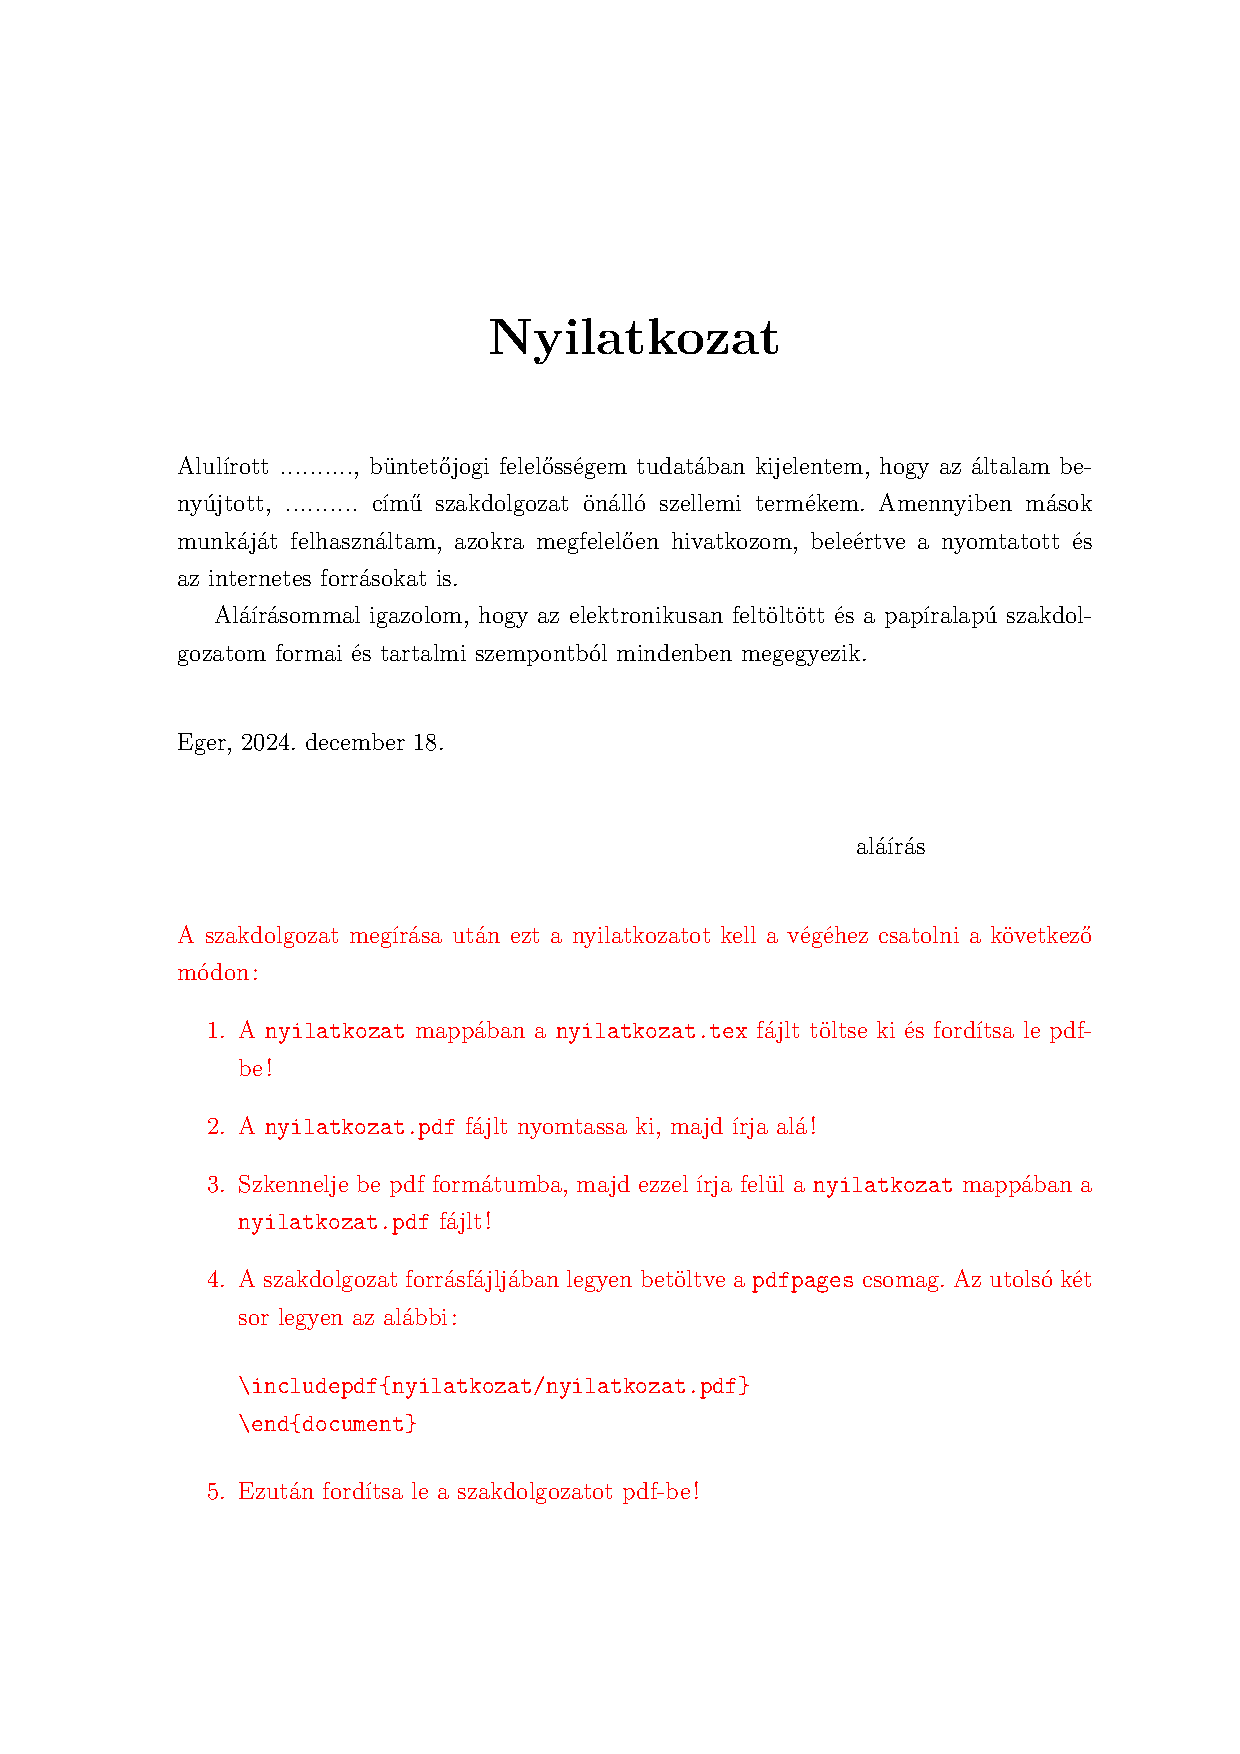
\includepdf{nyilatkozat/nyilatkozat.pdf}
\end{document}



